\chapter{Propuesta}\label{chapter:proposal}
La propuesta para el sistema de recuperación de información de imágenes basado en contenido comprende dos etapas principales y una etapa final de sistema de recuperaci\'on. La tarea de cada una de las etapas, en conjunto, posibilita lograr el objetivo principal, obtener relevancia para un conjunto de im\'agenes, desde una consulta en forma de texto en lenguaje natural. Para vincular conceptos en un mismo espacio, ya sea imagen o texto, se emplean embeddings (vectores multidimensionales) como contextos. Dada la naturaleza de estos vectores, ser\'a posible entonces, establecer una relaci\'on de similitud vectorial entre cualquier tipo de concepto que se encuentre en este formato de embeddings, en el caso particular de este trabajo, se pretende trabajar con conceptos de im\'agenes y texto.(ver diagrama \ref{fig:etapas})

\begin{figure}[H]
    \centering
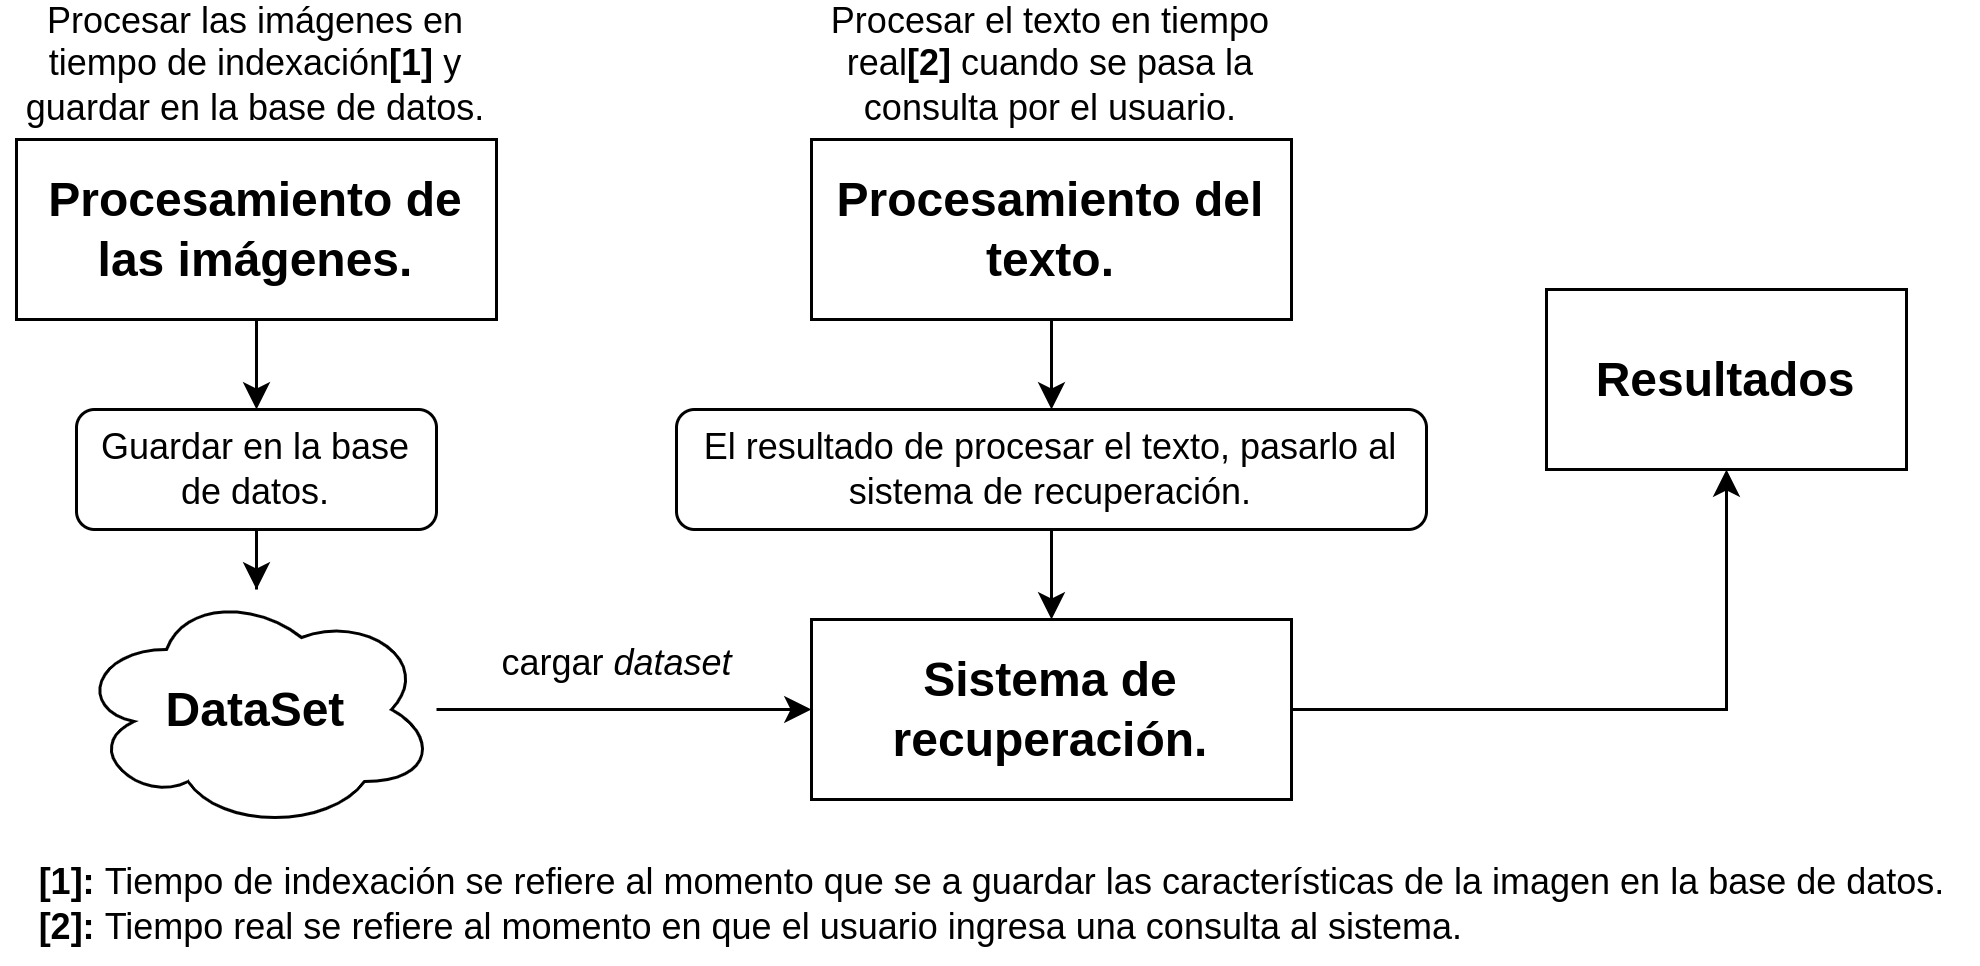
\includegraphics[height=0.25\textheight]{Graphics/Todas.drawio.png}
    \caption{Combinaci\'on de cada una de las etapas de la propuesta.}
    \label{fig:etapas}
\end{figure}    

\section{Etapas de la propuesta}

La primera etapa de procesamiento y extracción de características de la imagen tiene lugar durante el tiempo de indexación. Las características de las imágenes se procesan y almacenan en forma de vectores en el momento de generación de los datos. Posteriormente, utilizando estos vectores, se procede a recuperar la información en tiempo real mediante métodos mucho más rápidos y eficientes que los utilizados en tiempo de indexación. Este análisis de la imagen incluye diversas opciones y permite la ajustabilidad de parámetros para variar los resultados de acuerdo a lo que se determine más adecuado para lograr una mejor similitud entre contextos.(ver diagrama \ref{fig:etapa1})

\begin{figure}[H]
\centering
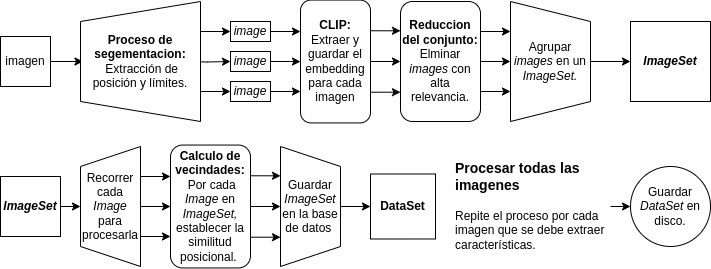
\includegraphics[width=\textwidth]{Graphics/Image.drawio.png}
\caption{Etapa de procesamiento de imagen.}
\label{fig:etapa1}
\end{figure}

La segunda etapa se encarga de procesar el texto proporcionado por la consulta de los usuarios. Esta etapa está compuesta por una variante implementada, y dos variantes propuestas. Está diseñada para ser escalable, lo que permite mejorar significativamente el procesamiento del texto en futuras implementaciones.(ver diagrama \ref{fig:etapa2})


\begin{figure}[H]
    \centering
    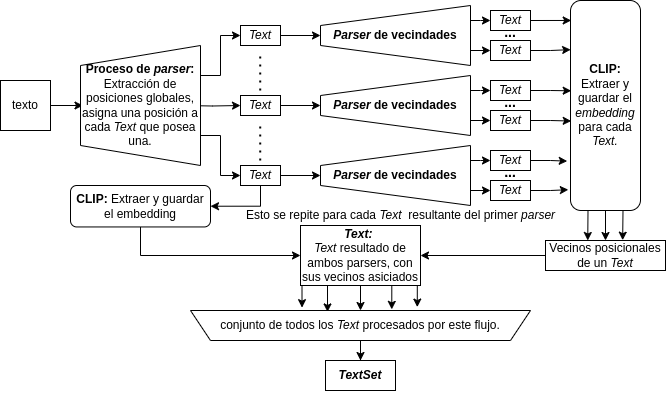
\includegraphics[width=\textwidth]{Graphics/Text.drawio.png}
\caption{Etapa de procesamiento de texto.}
\label{fig:etapa2}
    \end{figure}

La tercera y \'ultima etapa, es la encargada de recuperar datos relevantes para un concepto entrado por consulta. Potencialmente, los datos ser\'an im\'agenes y las consultas texto, no obstante, dado el enfoque planteado, los datos y la entrada pueden pertenecer a cualquier concepto del cual sea posible obtener su embedding. Un ejemplo de ello es que, con el mismo sistema de evaluaci\'on, se puede pasar por consulta tanto imágenes como textos, ya que ambos poseen embeddings como contexto.(ver diagrama \ref{fig:etapa3})

\begin{figure}[H]
\centering
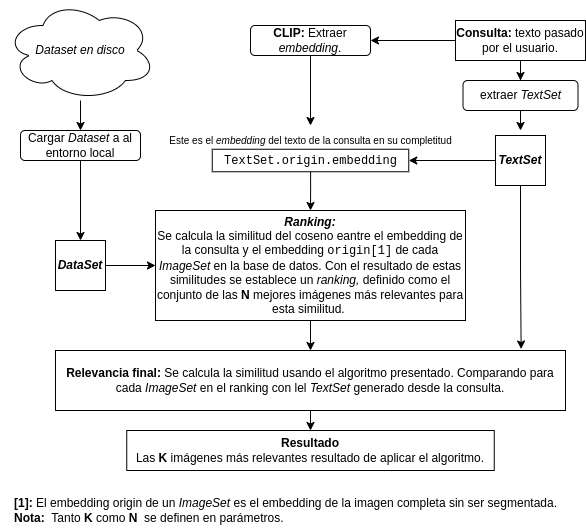
\includegraphics[height=110mm]{Graphics/SystemRetrieval.drawio.png}
\caption{Etapa del sistema de recuperaci\'on.}
\label{fig:etapa3}
\end{figure}


\section{Etapa de procesamiento de imagen}
Esta etapa se divide en tres variantes que, a su vez, poseen una base común como metodología, cambiando solo los conceptos que se emplean en cada una de estas. La metodología principal está dada por una serie de procesos que serán explicados en esta sección. Para facilitar la comprencion de esta, se definen dos conceptos fundamenales.

El primero es el concepto de \textbf{\textit{Image}}. Una \textit{Image} se define como un conjunto de características que se extraen de una imagen: un \textit{embedding}, una descripción, una posición, una serie de vecinos por posición relativa a esta imagen, y límites en los ejes coordenados. Los vecinos hacen referencia a las imágenes cercanas a la \textit{Image} en cuestión. Los límites definen la región rectangular donde se encuentra ubicada la imagen, dado que una imagen no siempre ocupa todo el espacio del plano. En la figura \ref{fig:imageexample} se muestra un ejemplo de una \textit{Image}, donde la imagen de referencia de la misma es la comprendida dentro del cuadro de segmentaci\'on. En la zona inferior a la imagen se definen sus caracter\'isticas.

\begin{figure}[H]
    \centering
    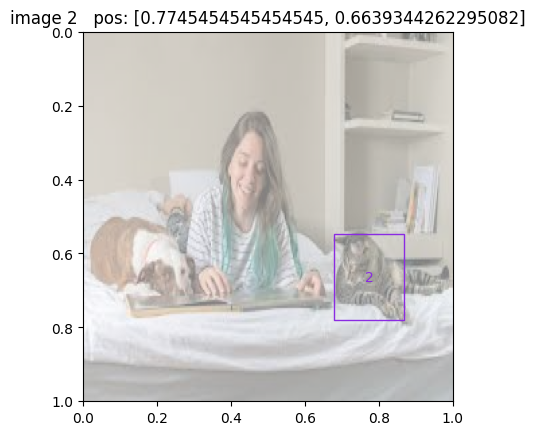
\includegraphics[height=0.3\textheight]{Graphics/ImageExample.png}
    \caption{Image}
    \label{fig:imageexample}
\end{figure}

(ver figura \ref{fig:neighbords}, visualizaci\'on de vecindades)
\begin{verbatim}
    embedding: [.........................................]    
    caption: None    
    position: (0.7745,0.6639)
    #definidos en el orden (top,right,bottom,left)
    limits: (0.56, 0.88, 0.76, 77)
    neigbords: #|Similar a figura
\end{verbatim}


El segundo concepto es \textbf{\textit{ImageSet}}. Un \textit{ImageSet} se define como un conjunto de \textit{Images} donde cada una de las imágenes de referencia de estos está relacionada con una misma imagen, una imagen general. Cada una de estas \textit{Images} constituye una segmentación de la imagen principal. En resumen, \textit{ImageSet} es el conjunto de características de una imagen subdividida en segmentaciones relacionadas, posicionalmente, entre s\'i. En la figura \ref{fig:imageset_example} se muestra un ejemplo de un \textit{ImageSet}, donde cada una de las segmentaciones representa un \textit{Image}, y el conjunto de todas estas conforman la lista de Images del \textit{ImageSet}. En la zona inferior a la imagen se definen sus caracter\'isticas.

\begin{figure}[H]
    \centering
    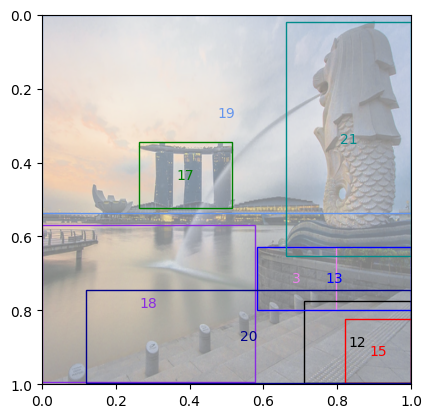
\includegraphics[height=0.3\textheight]{Graphics/ImageSetExample.png}
    \caption{\textit{ImageSet}}
    \label{fig:imageset_example}
\end{figure}
\begin{verbatim}
    origin: Image #imagen completa como Image    
    #Cada una de las imágenes comprendidas en un cuadro de 
    segmentación como Image
    Images: List[Image]     
\end{verbatim}


Con estos dos conceptos aclarados, se pasa a definir la metodología base para el procesamiento de imágenes. Inicialmente, para una imagen dada, se define un \textit{ImageSet} que será el encargado de agrupar todas las características de la imagen en una relación, en un conjunto. Para la extracción de características y procesamiento de la imagen, esta pasa a ser procesada y segmentada por un modelo de segmentaci\'on de im\'agenes. Este trabajo, en particular, utiliza el modelo de segmentación SAM (\textit{Segment Anything Model})[\cite{huggingface2022sam}]; dado la escalabilidad del código, este \'ultimo es perfectamente sustituible por otro modelo que se encargue de realizar la tarea de segmentaci\'on de imágenes. En trabajos futuros, ser\'a posible hacer uso de modelos más potentes o más rápidos que el integrado actualmente. El tamaño de las segmentaciones, así como los hiperparámetros del modelo SAM, son modificables. En caso de ser necesario, los par\'ametros del modelo pueden ajustarse a la problem\'atica que surja.

Terminada la tarea de segmentaci\'on de imagen, el paso que sigue, es descartar las imágenes que resultan ser semejantes a muchos conceptos muy distantes entre sí, las imágenes que son relevantes y afectan por ello los resultados esperados. Este proceso de descartar imágenes relevantes es muy importante para que los modelos usados no generen conceptos relevantes que resultan perdida de precisi\'on general. Para realizar este proceso se cuenta con un conjunto de conceptos muy distantes entre sí, un umbral a partir del cual se considera relevante una similitud, y un porcentaje que indica, cu\'ando una imagen posee una relevancia alta para el universo. Ergo, una imagen ser\'a descartada por alta relevancia, si resulta ser similar a una parte considerable del conjunto de conceptos distan mucho entre s\'i.

Una vez concluido este proceso, se encontrará en el \textit{ImageSet} definido al inicio, todo un conjunto de imágenes que lo conforman, cada una de las cuales será una imagen que contendrá, en este momento, un identificador, una posición relativa al espacio general, y los límites superiores e inferiores de cada eje del plano. Estos dos últimos se obtienen como resultado de aplicar el modelo de segmentación. Cada una de estas imágenes, están ahora relacionadas como conjunto, teniendo esta relación, sus posiciones y sus límites, el siguiente paso es establecer las relaciones de vecindad posicionales para las imágenes entre s\'i.

Para establecer esta relación se cuenta con etiquetas, ya que se espera que la descripción posicional sea por texto, las etiquetas entonces están acorde a ello, están acorde a lo que se espera como lenguaje natural. Las etiquetas son las siguientes:
\begin{itemize}
    \item \textbf{n}: Indica la cercanía a la posición superior relativa a la imagen. Dice que tan cerca está un vecino de la posición superior relativa a la imagen en cuestión.
    \item \textbf{s}: Indica la cercanía a la posición inferior relativa a la imagen. Dice que tan cerca está un vecino de la posición inferior relativa a la imagen en cuestión.
    \item \textbf{e}: Indica la cercanía a la posición derecha relativa a la imagen. Dice que tan cerca está un vecino de la posición derecha relativa a la imagen en cuestión.
    \item \textbf{w}: Indica la cercanía a la posición derecha relativa a la imagen. Dice que tan cerca está un vecino de la posición derecha relativa a la imagen en cuestión.
    \item \textbf{beside}: Indica la cercanía a la posición derecha o izquierda relativa a la imagen. Dice que tan cerca está un vecino de alg\'un lado de la imagen en cuestión.
    \item \textbf{ne}: Indica la cercanía a la posición derecha superior relativa a la imagen. Dice que tan cerca está un vecino de la posición a 45° de la imagen en cuestión.
    \item \textbf{nw}: Indica la cercanía a la posición izquierda superior relativa a la imagen. Dice que tan cerca está un vecino de la posición a 135° de la imagen en cuestión.
    \item \textbf{se}: Indica la cercanía a la posición derecha inferior relativa a la imagen. Dice que tan cerca está un vecino de posición a 315° de la imagen en cuestión.
    \item \textbf{sw}: Indica la cercanía a la posición izquierda inferior relativa a la imagen. Dice que tan cerca está un vecino de la posición a 225° de la imagen en cuestión.
    \item \textbf{in}: Indica que el vecino está dentro de la imagen en cuestión.
    \item \textbf{next}: Indica que el vecino está en una posición cercana a la imagen en cuestión.
\end{itemize}
Cada vecino será entonces, una relación etiqueta-(concepto, similitud), donde se hace referencia al concepto en la posici\'on dada, y se indica que tan similar es la posición con respecto a una etiqueta. Por ejemplo, ver figura \ref{fig:neighbords}.

La definición de la similitud posicional ha sido un tema muy cuestionable, dado que se busca similitud entre lenguaje natural e imágenes. Definir entonces, qu\'e tan similares son las posiciones entre imágenes, está estrechamente relacionado con la interpretación de cómo se puede pretender explicar posiciones a nivel de lenguaje natural y cómo se espera la salida para ello.

\begin{figure}[H]
\centering
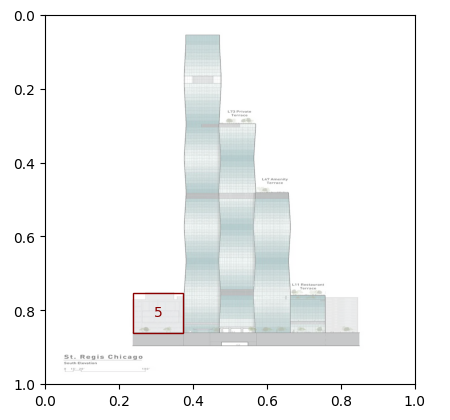
\includegraphics[height=80mm]{Graphics/building.png}
\caption{Interpretaci\'on de relaciones espaciales}
\label{fig:edificio}
\end{figure}

Un ejemplo claro de que la definición de posición está ajustada a la interpretación del observador sería una imagen en la que se ve un edificio. En \textit{Figura \ref{fig:edificio}} se podría decir que el edificio está a la derecha de la \textit{Image 5}[figura \ref{fig:edificio}], porque en realidad lo está, en su base coinciden. También se podría decir que el edificio está arriba, en la posición superior de la \textit{Image 5}. Y, evidentemente, el edificio parece estar en la zona superior derecha de la \textit{Image 5}. Se interpreta cada una de estas posiciones, definir que posici\'on es mejor sigue siendo un problema de interpretaci\'on del observante.

Como respuesta a esta ambigüedad se plantearon varias métricas o alternativas para poder decidir qué usar. Por ejemplo, la métrica que utiliza distancias angulares dudará que el edificio está completamente ubicado en su derecha, mientras que las otras interpretarán que hay un edificio en su derecha con una similitud perfecta. Las métricas usadas se definen a continuación.

\subsubsection{Ángulo entre los centros y Distancia entre los extremos}

Para el c\'alculo de esta similitud se definen las siguientes variables:
\begin{itemize}
    \item $d =$ Distancia euclideana entre las im\'agenes. Esta se calcula como la distancia m\'inima entre los l\'imites de las \textit{Images}.

    \item $a =$ \'Angulo entre el centro del \textit{Image} y el centro del \textit{Image} vecino.

    \item $b =$  El ángulo correspondiente a la posición dada, con respecto a la imagen, por ejemplo, para la posición derecha superior, se espera que el ángulo esté cerca de los 45 grados.

    \item $u =$  Umbral multiplicador de resultado, con ello se ajusta la salida como se desee.
\end{itemize}
Con estas variables definidas, donde para cada posici\'on var\'ia el valor del $b$ esperado, se llega a que la similitud posicional propuesta ser\'a:

\[sim_pos = (1-d)*(1- |a-b|/2*\pi) * u \]

\subsubsection{Reescalado las imágenes.}

Esta alternativa usa la misma idea de la anterior, solo que ahora, antes de calcular la distancia angular, se reescalan las imágenes a una misma dimensión. De esta manera se consigue que las posiciones sean más importantes que las escalas de los objetos que se analizan. Ahora un objeto con mucho más escala que otro se ajustará al pequeño para definir sus posiciones relativas. En caso del ejemplo anterior, \textit{Figura \ref{fig:edificio}}, el edificio estar\'a a la derecha de la \textit{Image 5}, pero no se considerar\'a en zona superior porque la base en el eje horizontal es la misma, es decir, parten de la misma posici\'on. Esta es una manera interpretar relaciones posicionales, por eso ha sido planteada como una variante.

\subsubsection{Alternativa de pesos en los ejes coordenados.}

Esta alternativa calcula la distancia entre los objetos tanto en el eje vertical como en el horizontal. Tanto al eje principal como al secundario se le asignara un pes de importancia que, ajustara la distancia de este eje. El eje principal ser\'a el de desplazamiento de la posici\'on indicada, por ejemplo, si se está analizando un objeto a la derecha o a la izquierda, entonces el eje principal será el eje horizontal, ya que de derecha a izquierda el desplazamiento es horizontal, y el secundario será el vertical. Teniendo esto en cuenta se ajustan los parámetros a conveniencia de tal forma que se acerque al mejor resultado posible, descrito posicionalmente. Cada uno de los parámetros ajustables correspondientes a esta función son los siguientes.

\begin{itemize}
    \item \textbf{Multiplicador de posiciones relativas:} Este parámetro se usa para ajustar con un multiplicador los valores de las posiciones relativas entre objetos, es decir, el resultado de calcular la similitud posicional es modificado por este multiplicador, dando m\'as o menos importancia a este proceso. 

    \item \textbf{Importancia distancia en el eje no principal:} Define qué tan importante se considera la cercanía o lejanía en el eje no principal de una vecindad. Por ejemplo, si se est\'a trabajando en una vecindad izquierda o derecha, el eje no principal será el vertical, el eje $y$. Una vez se tiene la distancia del eje no principal, se eleva este resultado a la potencia del valor indicado por este par\'ametro.

    \item \textbf{Importancia distancia en el eje principal:} Define qué tan importante se considera la cercanía o lejanía en el eje principal de una vecindad. Por ejemplo, si se est\'a trabajando en una vecindad izquierda o derecha, el eje principal será el horizontal, el eje $x$. Una vez se tiene la distancia del eje principal, se eleva este resultado a la potencia del valor indicado por este par\'ametro.
\end{itemize}

A continuación se muestran valores de similitud por vecindad para dos métricas distintas, mostrando la similitud de los vecinos para la \textit{imagen 3}. Estos resultados son ajustables cambiando valores de parámetros espec\'ificos. La etiqueta define la posición relativa a la imagen en cuestion, en este caso la imagen 3, cada valor está compuesto por dos elementos, la referencia a la imagen en la posici\'on 0, y en la posici\'on 1, el valor de semejanza de sus posiciones con relación a la zona de la imagen que le corresponde, esta zona est\'a definida por la etiqueta.

%\begin{figure}[h]
\begin{figure}[H]
\centering
 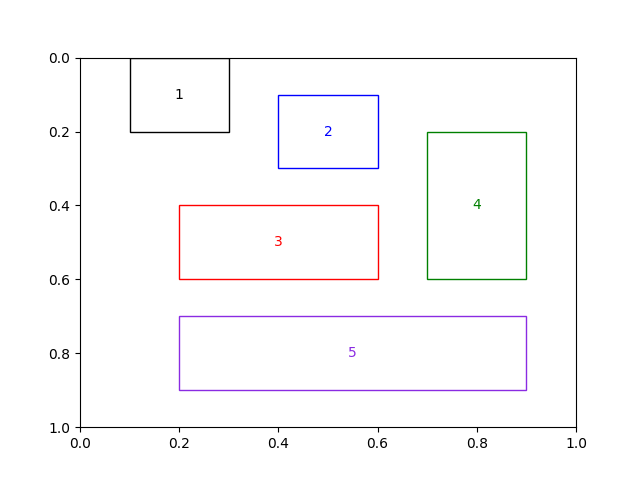
\includegraphics[width=\textwidth]{Graphics/regions.png}
\caption{\textit{ImageSet} de prueba para observar vecindades.}
\label{fig:neighbords}
\end{figure}

\noindent\textbf{\'Angulo entre los centros y Distancia entre los extremos}
\begin{verbatim}
Image3 Neighbords using angle_similarity
 w: [(image 1, 0.2291)]
 e: [(image 4, 0.7596), (image 5, 0.2656)]
 n: [(image 1, 0.5638), (image 2, 0.7156), (image 4, 0.1559)]
 s: [(image 5, 0.6343)]
 nw:[(image 1, 0.4583)]
 ne:[(image 4, 0.2807)]
 sw:[]
 se:[(image 5, 0.5313)]
 in:[]
 beside: [(image 1, 0.2062), (image 4, 0.6836), (image 5, 0.2390)]
 next: [(image 5, 0.6343), (image 1, 0.5638), (image 2, 0.7156), 
        (image 4, 0.7596)]
\end{verbatim}

\noindent\textbf{Alternativa de pesos en los ejes coordenados}
\begin{verbatim}
Image3 Neighbords using weights_similarity
 w: [(image 1, 0.4734)]
 e: [(image 4, 0.9369), (image 5, 0.5694)]
 n: [(image 1, 0.6555), (image 2, 0.9369), (image 4, 0.5694)]
 s: [(image 5, 0.9369)]
 nw: [(image 1, 1.1289)]
 ne: [(image 4, 1.5063)]
 sw: []
 se: [(image 5, 1.5063)]
 in: []
 beside: [(image 1, 0.4734), (image 4, 0.9369), (image 5, 0.5694)]
 next: [(image 5, 1.5063), (image 1, 1.1289), (image 2, 0.9369),
        (image 4, 1.5063)]
\end{verbatim}
La segunda alternativa no tiene en cuenta las dimensiones de las segmentaciones para calcular la posición relativa. En la primera métrica, si una imagen es más alta, est\'a más extendida en el eje $y$, entonces su ángulo relativo a otra varía según la escala de la misma.

Sobre la base de la metodolog\'ia planteada, se proponen tres variantes para ser utilizadas como conceptos, entre los cuales, poder hallar relevancia mediante cálculos de similitud.

\subsection{Uso de descripciones de las imágenes}
Este método propone generar la descripción de la imagen en lenguaje natural. Con texto en lenguaje natural hallar la similitud directamente sería una opción válida, pero esta no es considerada en un primer momento, dado que un trabajo vago sobre el lenguaje natural no nos garantiza una buena precisión al momento de hallar similitud. Como alternativa a esto se usan embeddings del texto, generados con modelos potentes de visión artificial que están diseñados para generar embeddings multimodales. En el caso particular de este proyecto se usa el modelo CLIP[\cite{clip}] que permite generar embeddings tanto desde texto como desde imágenes, vectores de 512 dimensiones. El proceso completo de esta metodología sería entonces generar descripciones desde la imagen, desde esta descripción generar un embedding y usar este último como contexto que se compare para hallar similitud entre este y los embeddings generados desde el texto de la consulta.

Este proceso requiere de modelos diseñados para describir imágenes en lenguaje natural, modelos como son BLIP[\cite{blip}], BLIP2[\cite{blip-2}], LLaVA[\cite{llava}] y GPT4-V.[\cite{gpt-4v}] El proceso de generar descripciones suele ser lento según el modelo que se utilice, los modelos más potentes requieren de un hardware, de GPU, muy potente. En el caso de este proyecto se utiliza BLIP[\cite{blip}] para generar descripciones, también cuenta con el modelo BLIP2 integrado, pero no es utilizado debido a su exigencia de hardware y la insuficiencia del mismo.

Como todo modelo de Machine Learning, estos modelos están sujetos a errores y tienen sus puntos fuertes y débiles. Por lo general, imágenes poco claras generan textos con conceptos muy alejados a lo esperado, por ello se suelen perder algunas segmentaciones que se consideran importantes. No obstante, la gran mayoría de las imágenes como estas suelen ser desechadas por tener mucha relevancia.

\subsection{Uso de embedding de las imágenes}
La segunda variante es la que, actualmente, se usa por defecto en el proyecto, dado que es más ligera y alcanza los mejores resultados entre las tres variantes planteadas.

Esta variante implica tomar la imagen segmentada, procesarla en un modelo generador de embeddings, se usa CLIP, y usar este embedding como concepto para hallar similitud. Dado que CLIP[\cite{clip}] está diseñado para generar embeddings para imágenes y para textos en el mismo espacio, esto es muy útil para usar este mismo generador para ambas partes y poder comparar similitud entre ellos.

El proceso de generar embeddings con CLIP[\cite{clip}] es considerablemente rápido, tardando, \textit{grosso modo}, 20 ms[\cite{BuildingImageClip-20ms}] para generar el embedding de una imagen con una GPU v100; se puede decir que es aún más rápido en cuanto a su velocidad relativa a modelos generadores de descripciones, que suelen tardar varios segundos, dependiendo del modelo específico que se use. El proceso de generación de embeddings con CLIP[\cite{clip}] , si bien est\'a expuesto a fallos o salidas no esperadas, suele ser más preciso que utilizar un modelo generador de descripciones al alcance del hardware disponible o la disponibilidad del modelo, dado que los más potentes no son código abierto. Se desconoce que tan preciso puede ser usar el modelo GPT4-V[\cite{gpt-4v}], el cual es muy potente en este campo, como también se desconoce que tan preciso sería usar CLIP-2[\cite{clip2-paper}]para generar embeddings, ambos modelos son de código cerrado de OpenIA.

\subsection{Combinaci\'on de ambos modelos}
La tercera variante es combinar ambas variantes anteriores. De esta forma, el cálculo de la similitud sería entonces la media de la similitud por texto y la similitud por imágenes. Esta variante suele ser tan precisa como los modelos de descripción que se usan para su descripción, pero exige mucho hardware con el cual no se cuenta. Eso hace dif\'icil utilizar modelos más potentes que BLIP[\cite{blip}].

\section{Etapa de procesamiento de texto}

Esta etapa consiste en extraer características del texto ingresado por consulta. Específicamente, características posicionales indicadas con lenguaje natural. Para ello, se desea que, para un texto de entrada en lenguaje natural, se genere una serie de textos parseados por posiciones descritas, equivalente a lo que se hace en la etapa 1 con las imágenes. El proceso de obtener posiciones en el texto suele ser más engorroso que en el procesamiento de las imágenes, dado que en el caso de las imágenes, al ser segmentadas, cada una de estas segmentaciones posee la información posicional en el plano de sí misma. En el caso del lenguaje natural es necesario parsear lo que expresa un usuario en una consulta. La etapa del procesamiento del texto de la consulta, a diferencia de la etapa de procesamiento de la imagen, ocurre en tiempo real en el momento de la consulta, ergo debe ser considerablemente rápida para que cumpla con las expectativas.

Al igual que en la etapa de procesamiento de imágenes, aquí también se definirán dos conceptos fundamentales para comprender la metodología utilizada.

El primero es el concepto de \textit{\textbf{Text}}. Un \textit{Text} se define como un conjunto de características que se extraen de un texto, las cuales son: un \textit{string}, un embedding, una posición y una serie de vecinos por posición relativos a este. Los vecinos hacen referencia a la cercanía entre conceptos. Por ejemplo, para el texto en lenguaje natural \textit{In top right side of the image there are a dog next to a cat sleeping on a couch}, se espera un \textit{Text} de la siguiente forma:

\begin{verbatim}
    text.string = 'a dog next to a cat sleeping on a couch.'
    text.pos = (0.5, 0.5)
    text.neighbors[next] = 'cat sleeping on a couch'
\end{verbatim}

Para mejor comprensi\'on del lector, se debe asumir que las posiciones van desde $[(-1,1), (1,1)]$.

El segundo concepto es \textit{\textbf{TextSet}}. Un \textit{TextSet} se define como un conjunto de \textit{Texts} donde cada uno representa una subdivisi\'on de un \'unico texto general, además, también posee un \textit{Text} que hace referencia al texto original. En pocas palabras, \textit{TextSet} es el conjunto de textos que conforman el texto original, separados por puntos o por posiciones indicadas con lenguaje natural.

Para esta etapa de procesamiento de lenguaje se plantean 3 variantes posibles, de las cuales, una ha sido implementada.

\subsubsection{Análisis sintáctico y parser}
La variante principal e implementada en el proyecto es el uso de un parser para lenguaje natural con el fin de parsear contenido que haga referencia a relaciones posicionales. El lenguaje natural es ambiguo, un parser diseñado sobre este no será perfecto, pero puede abarcar una gran parte de las estructuras gramaticales que forman, de alguna manera, la definición de posiciones a través de texto.

Esta alternativa tiene como principal punto débil la ambigüedad del lenguaje, ergo, en algunos casos muy particulares, el proceso de parser no nos dará la salida esperada. Como punto fuerte se puede decir que esta alternativa tiene un alto nivel de escalabilidad. Cada vez que se quiera definir una nueva regla gramatical es posible hacerlo, dado que el lenguaje ya es, por naturaleza, ambiguo, una nueva regla gramatical no afectará en este aspecto. Siempre que se agregue una nueva regla, esta no debe generar conflictos graves con las anteriores.

Para la implementación de este sistema de parser se usa la biblioteca \textit{SLY (Sly Lex Yacc)}[\cite{sly}]. Esta biblioteca está diseñada para realizar análisis léxicos y sintácticos para lenguajes de programación, no está exactamente diseñada para este tipo de gramática ambigua, pero se logra adaptar a las necesidades y al uso que se le da.

El análisis de un texto está dividido en dos fases, la primera fase de tokenización, y la segunda fase de análisis sintáctico o parser. Los tokens están definidos según la necesidad de buscar patrones comunes para describir posiciones en imágenes. Cada una de las palabras del texto serán procesadas por un análisis léxico que definirá si esta es token o palabra común. Dado que en el lenguaje natural todas las palabras pueden ser parte de otro texto, las palabras coincidentes con los tokens no siempre serán uno de estos, es decir, que una palabra esté en el grupo de tokens no implica que sea un token necesariamente. Una palabra es un token, si y solo si, está contenida en un patrón que constituye una regla gramatical en su completitud y, este patr\'on no genera conflictos con otros patrones anteriormente analizados y seleccionados como tokens; de esta forma solo se consideran tokens los patrones que se usan para describir relaciones posicionales. 

Seguido a esta fase de tokenización est\'a la fase de análisis sintáctico. Esta fase encarga de parsear todo el texto por relaciones posicionales en caso de que se especifiquen las mismas. Este análisis sint\'actico o parser, está dividido en dos subetapas, dos parsers distintos. El primer parser consiste en un análisis para las relaciones globales de los objetos con respecto a la imagen, y e segundo análisis se encarga de las relaciones posicionales relativas entre conceptos.

\subsubsection{Parser de posiciones globales}

En un primer momento se parsean las posiciones globales, las posiciones de un objeto respecto a la imagen en su totalidad, de esta forma se obtiene la posición de cada \textit{Text} que conformará el \textit{TextSet}. Para ello se definen algunas reglas gramaticales que se usan en el lenguaje natural para expresar posición en el espacio, o relativa a la imagen. Por ejemplo, para la frase: \textit{'there are a dog next to a ball in top of image'}, se parsea a través de la regla \textit{'IS text ON pos OF IMAGE'}, de esta forma se obtiene un \textit{Text} con \textit{string} igual a \textit{'dog next to a ball'} y posici\'on, \textit{grosso modo}, igual a $(0, 0.66)$. En un primer momento, el tokenizador o analizador léxico referente a este análisis de posiciones globales posee como tokens los siguientes:

\begin{verbatim}
tokens = [ON, TO, OF, AND, IS, POS, POSITION, IMAGE, WORD, NEXT]
\end{verbatim}

Cada uno de estos es representado por una palabra clave que puede corresponder a ellos, no poseen una palabra única para cada token, un token puede estar representado por más de una palabra, y cada una de estas cuando aparezca en el texto, puede representar un token de los anteriores. Las palabras claves representan un token dado, el conjunto de palabras claves es perfectamente extensible, solo se debe agregar a este una nueva palabra clave y esta ser\'a entonces tratada como posible token.

\begin{verbatim}
keywords = {
        ON = [ in, on, at, near, find…],
        OF = [ of ],
        TO = [ to ],
        AND = [ and ],
        IS = [ is, are, there's, find …],
        POS = [ left, right, buttom, bottom, top, down, up, 
        lower, center, middle, corner…],
        POSITION = [ position, side, location…],
        IMAGE = [ image, picture, photo…],
        NEXT = [ next, near ]
        }
\end{verbatim}

Durante la fase de tokenización, cada palabra en el texto se somete a un proceso para determinar su tipo de token. Este proceso implica verificar si la palabra coincide con un patrón posible en la gramática. Si la palabra cumple con este criterio, se clasifica como un token; si no, se designa como una palabra común o WORD.

Posteriormente, en la fase de análisis sintáctico, se define la gramática de las relaciones espaciales, la cual se considera el pilar fundamental del procesamiento de texto. Este análisis se basa en la identificación de patrones gramaticales que permiten expresar relaciones espaciales en el texto. Las reglas gramaticales han sido definidas siguiendo la siguiente gram\'atica.
 
\begin{verbatim}
WORD ::=  WORD
        | Any
    
pos ::=  POS
       | POS POSITION 

text ::=  WORD
        | [text]+
        
relation ::=  ON pos IS text
            | ON pos OF IMAGE IS text
            | ON pos text
            | IS text ON pos OF IMAGE
            | IS text ON pos ","
            | IS text ON pos !OF
            | text ON pos !OF
            | text ON pos OF IMAGE
            | ON pos "," IS text
            | ON pos OF IMAGE "," IS text
            | ON pos OF IMAGE "," text
            | ON pos "," text
\end{verbatim}

\textbf{!TOKEN} indica que en ese patr\'on no puede haber un token tipo TOKEN en esa posici\'on. N\'otese que, en el caso de \textit{'IS text ON pos !OF '}, la ausencia de !OF al final podría generar conflictos de ambigüedad y hacer que palabras necesarias sean descartadas. \textbf{[TOKEN]|+} indica que el token se repite una o m\'as veces. \textbf{Any} se refiere a un token cualquiera que sea tratado como palabra.

En la segunda parte del parser, se analizan las posiciones relativas de los objetos entre sí. Al igual que en el caso anterior, existen una serie de reglas definidas para esto. Por ejemplo, para el texto \textit{'dog next to a ball'}, el parser seguirá la regla \textit{' text NEXT TO text'}. De esta forma, se espera obtener un text con \textit{string} igual a \textit{ 'dog' }, \textit{neighbors['next'] = 'a ball' }.

El proceso de parser y tokenizaci\'on, es igual al anterior, solo cambian las reglas gramaticales, y tokens no necesariamente id\'enticos. Por ejemplo, el token \textit{Image} no existe en esta an\'alisis. La gram\'atica del parser est\'a definida por las reglas, tokens y palabras claves definidos a continuaci\'on.
\begin{verbatim}
Tokenization
tokens = [ON, OF, AND, IS, POS, POSITION, WORD, NUM, TO, NEXT]

keywords = {
        ON = [in, on, at, find]
        OF = [of]
        AND = [and]
        IS = [is, are, theres, find]
        POSITION = [position, pos, side,location]
        NEXT = [next]
        TO = [to]
        POS = [ left, right, bottom, top, down, up, lower, center,
        middle, corner, near, bellow, front, beside ...]
    }

Gramatic    
WORD ::=  WORD
            | Any
    
pos ::=  POS
           | POS POSITION 

text ::=  WORD
            | [text]+
relation ::=   IS text ON pos OF text
            | IS text TO pos OF text
            | IS text ON pos TO text
            | IS text TO pos TO text
            | text ON pos TO text
            | text ON pos OF text
            | IS text , pos TO text
            | IS text , pos OF text
            | IS text pos TO text
            | IS text pos OF text
            | text pos TO text
            | text pos OF text
            | IS text NEXT TO text
            | IS text NEXT OF text
            | text NEXT OF text
            | text NEXT TO text
            | ON text pos , IS text
            | ON text pos , text
            | ON text pos IS text
            | ON pos OF text , IS text
            | ON pos OF text , text
            | TO pos OF text , IS text
            | TO pos OF text , text
            | ON pos TO text , IS text
            | ON pos TO text , text
            | TO pos TO text , IS text
            | TO pos TO text , text
            | ON pos OF text IS text
            | TO pos OF text IS text
            | ON pos TO text IS text
            | TO pos TO text IS text
            | pos TO text , IS text
            | pos TO text , text
            | pos OF text , IS text
            | pos OF text , text
            | pos TO text IS text
            | pos OF text IS text
            | NEXT TO text , text
            | NEXT OF text , text
            | NEXT TO text IS text
            | NEXT OF text IS text
\end{verbatim}

\subsubsection{Otras variantes de procesamiento de texto }
Se ha considerado el uso de un \textit{Large Language Model} (LLM) para procesar los textos de las consultas. A través de una API se describiría el sistema del parser deseado, y se esperaría que este, se encargue de parsear el texto. Modelos como GPT-3[\cite{gpt3} podrían ser una opción viable. Sin embargo, se ha intentado reentrenar modelos de lenguaje para pasarles entradas y salidas, pero estos no han tenido éxito debido a que no están diseñados para devolver siempre la misma respuesta para una misma entrada. Por lo tanto, no es posible entrenarlos con este objetivo. Los modelos que han fallado en este aspecto incluyen GPT-2[\cite{gpt2}], BERT[\cite{bert}] y T5[\cite{t5}].

Otra alternativa v\'alida es la creación de un modelo propio que se encargue de procesar texto y devolver relaciones posicionales de este. Dado que se dispone de un parser, del cual se conoce qu\'e patrones en un texto encontrará resultados correctos. Con esta información, se puede conformar una gran parte de un enorme conjunto de datos de forma automática, utilizando modelos de lenguajes actuales como GPT-3[\cite{gpt3}]. Al describir al modelo, el tipo de estructura gramatical que se sabe, es correcta, se pueden generar muchos casos de entrenamiento que ser\'an correctamente procesados por el parser. En combinación de estas dos condiciones, se generarán grandes cantidades de datos de manera automática. Este modelo tiene la ventaja de que el \textit{dataset} puede ser ampliado con casos, para los cuales el parser pueda fallar, permitiendo así aprender tambi\'en de estos. Incluso se pueden crear diferentes parsers que no sean ambiguos entre sí para generar casos de prueba. Adem\'as, gracias al proceso de tokenizaci\'on, tambi\'en se tiene una relaci\'on de importancia para cada palabra, lo cual puede constituir una capa de atenci\'on que se centra, principalmente, en los tokens pertenecientes a la gram\'atica.

Una propuesta para este modelo ha sido creada, pero aún no ha sido entrenada. El modelo está implementado en tensorflow.keras, y est\'a constituido por las siguientes capas:

\begin{itemize}
    \item Dos capas de entrada, una para los tokens y otra para la atención que se le debe prestar a estos.
    \item Dos capas de \textit{Embedding} que convierten los tokens a un espacio de \textit{embedding}.
    \item Dos capas \textit{Cov1D} que son utilizadas para aprender patrones.
    \item Una capa de \textit{Attention}, para recibir las entradas y generar pesos seg\'un la atenci\'on que se deba prestar a cada token.
    \item Dos capas \textit{GlobalAveragePooling1D} para redimensionar el espacio a una dimensión.
    \item Una capa \textit{Concatenate}, para concatenar ambas capas superiores.
    \item Una capa \textit{Dense} de 256 dimensiones.
    \item Una capa \textit{Dense} de 512 dimensiones.
    \item Una capa \textit{Dense} de 1024 dimensiones.
    \item Una capa \textit{Dense} con cantidad de dimensiones igual a la longitud de la salida.
    \item Una capa \textit{Reshape} para ajustar la salida al formato de matriz deseado.
\end{itemize}
Las primeras 6 capas del modelo están basadas en la documentación oficial de TensorFlow[\cite{tensorflow}] para el uso de capas de atención, las capas de atenci\'on son las metodolog\'ias m\'as fuertes y m\'as utilizadas en el procesamiento del lenguaje natural. A partir del a\~no 2017, cuando fue publicado \textit{Attention is all you need}[\cite{transformers}], el procesamiento del lenguaje natural se ha inclinado a esta arquitectura.

\begin{figure}[H]
\centering
 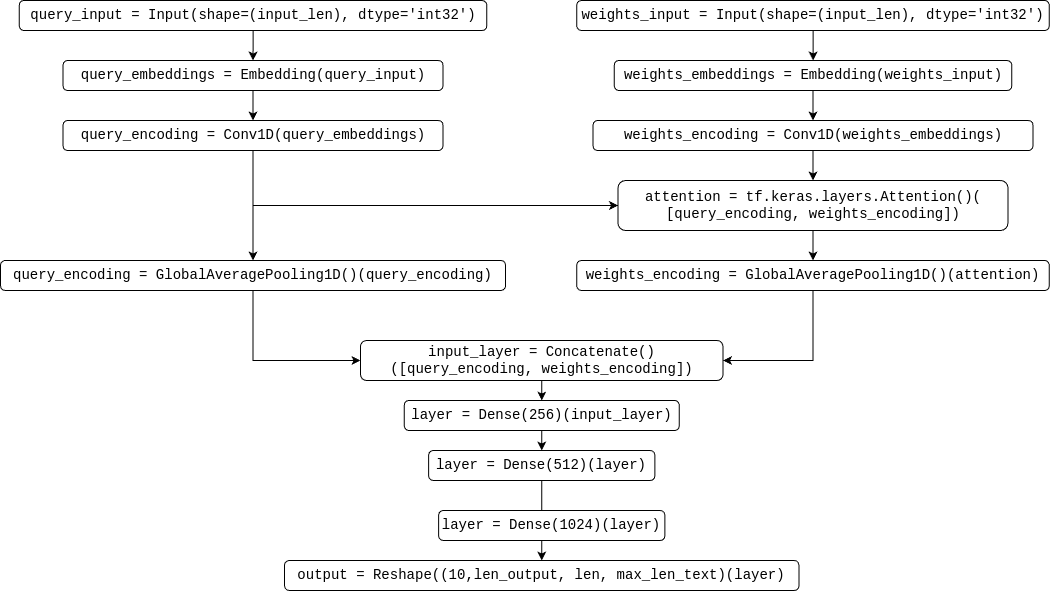
\includegraphics[width=\textwidth]{Graphics/model.png}
 \caption{Modelo en Keras}
 \label{fig:modelo}
\end{figure}

\subsection{Etapa de cálculo de similitud y recuperación de información}

Después de las dos etapas anteriores, que implican el procesamiento de imágenes durante la indexación y el procesamiento de texto en tiempo real, se procede a calcular la similitud entre el texto proporcionado en la consulta y las imágenes de la base de datos.

Para calcular la similitud entre un \textit{Text} y una \textit{Image}, se siguen los siguientes pasos:
\begin{itemize}

    \item  Se calcula la similitud del coseno entre el embedding del \textit{Text} y de la \textit{Image}: 
    \[sim_{cosine} = 1- cos(v1,v2)/||v1||v2||\]

    \item  Se calcula la similitud por posici\'on, para ello se multiplica el valor de la similitud del coseno por la similitud posicional m\'as uno, para $v1$ y $v2$ vectores de posici\'on y $K$ un p\'arametro ajustable, la similitud posicional est\'a dada por la forma: 
        \[sim_{pos} = K- \sqrt((v_1.pos.x - v_2.pos.x)^2+(v_1.pos.y - v_2.pos.y)^2).\]
    Luego, la similitud final para un concepto en una posici\'on dada distinta de \textit{None}, estar\'a dada por la f\'ormula
            \[sim_{inpos} = sim_{cosine} *(sim_{pos}+1)\]
    
    \item Si el \textit{Image} y el \textit{Text} poseen similitud suficiente, es decir, una similitud superior a un umbral que determina si es relevante, entonces se avanza al siguiente paso. Se pregunta por cada vecino en la posici\'on $p$ relativa al \textit{Image} la similitud de este con cada vecino en la posición $p$ relativa a \textit{Text}. Por cada vecino en posici\'on $p$ en \textit{Text}, se guardar\'a el mejor, el m\'as relevante de los vecinos en la posici\'on $p$ de \textit{image}. Cada uno de los resultados obtenidos de este proceso se suma a la similitud final. Si el mejor de los resultados para una posición $p$ está por debajo de un cierto umbral, entonces significa que no hay nada semejante a lo que se espera en la posición indicada, por lo que la similitud entonces, disminuirá.

    \begin{verbatim}
        for neighbord in Text.neigbords:
            sim_inpos = sim_inpos(neigbord, Image.neighbords)
            if max(sim_inpos) > umbral:
                sim_region = max(sim_inpos))
            else:
                sim_region = max(sim_inpos) - umbral
            end_sim_region+= sim_region
        sim = sim_inpos(Text, Image)*(1+ end_sim_region)
    \end{verbatim}
            
    \item La similitud final est\'a dada por la similitud entre un \textit{ImageSet} y un \textit{text feaure}, es decir por un conjunto de \textit{texts} y un conjunto de \textit{Images}. Cada \textit{Text} halla similitud con cada una de las \textit{Images} si esta similitud relevante, entonces se guarda. Luego de recorrer todas las im\'agenes, la similitud para el \textit{Text} ser\'a la mejor de todas las similitudes con cada una de las \textit{Images}. La similitud final, es entoces, la suma de cada una de las similitudes por cada \textit{Text} en \textit{TextSet}. Esto garantiza que una descripci\'on detallada y precisa de la imagen, encuentre, en caso de existir, im\'agenes muy relevantes a la descripci\'on posicional.
        
        \[\sum(sim(Text_i, ImageSet) | sim_i>umbral\]
    

\end{itemize}

Como se ha mencionado, los parámetros utilizados para los cálculos de similitud, distancias, importancia y características son modificables. Esto permite buscar un mejor equilibrio de similitud, si es necesario. Esta flexibilidad mantiene una arquitectura escalable que no requiere cambios en métodos o clases para variar los resultados. A continuación se presentan estos parámetros.
\begin{itemize}
    \item \textbf{umbral de importancia de la distancia euclideana}(\textit{float}): Elevar a la potencia la distancia euclideana. Este valor define la imporatncia que se le da a las posiciones globales.
    \item \textbf{umbral de divisi\'on de la distancia euclideana}(\textit{float}): se divide el valor de la distancia euclineada por el valor de este par\'ametro.
    \item \textbf{similitud m\'inima relevante para regiones vecinas}(\textit{float}): Si la similitud es menor que este valor, se considera poco relevante y, en caso de que todas las relaciones posicionales sean poco relevantes, la similitud de la imagen va a disminuir para una descripci\'on dada.
    \item \textbf{similitud m\'inima relevante}(\textit{float}): Esta es la similitud a partir de la cual puede considerarse relevante un concepto, se utiliza en el \'ambito general, la relevancia posicional y general no tienen que depender una de la otra.
    \item \textbf{similitud m\'inima relevante original}(\textit{float}): Esta es la similitud a partir de la cual puede considerarse relevante la similitud entre la imagen original y el texto original.
    \item \textbf{similitud m\'inima relevante usando descripciones}(\textit{float}): Esta es la similitud a partir de la cual puede considerarse relevante una comparación a nivel de texto contra texto. 
    \item \textbf{uso de regiones negativas} (\textit{bool}): Define si las regiones pueden aportar efecto negativo a la similitud, en el caso de cercan\'ia entre un objeto y otro.
    \item \textbf{importancia de las regiones negativas}(\textit{float}): Define qu\'e tan importante es una regi\'on negativa, mientras m\'as alto, m\'as baja ser\'a la similitud de una regi\'on poco relevante.
\end{itemize}

\section{Otras Propuestas}

Una propuesta inicialmente considerada fue mejorar el reconocimiento de colores en la imagen, esta finalmente fue abandonada. Se decidió centrar más interés en la propuesta de reconocimiento posicional, ya que CLIP[\cite{clip}] maneja eficientemente las relaciones de colores en las imágenes, y por el contrario, no es tan competente en el manejo de las relaciones posicionales.

El análisis de colores es una propuesta válida que implica un análisis exhaustivo de las segmentaciones para determinar de manera óptima a qué objeto pertenece un color. Sin embargo, para implementarlo, se requiere trabajar con máscaras como forma de segmentación y definir combinaciones de embeddings junto con el color. Aunque CLIP[\cite{clip}] no es particularmente eficaz en la generación de embeddings para las máscaras, no está claro si esto mejoraría los resultados. Si se opta por utilizar otro modelo generador de embeddings se tendrían que implementar más formas de similitudes en las que el modelo actual no es bueno, probablemente, para esos nuevos modelos, el dise\~no de esta propuesta resultaría en mejores resultados.

\begin{figure}[H]
\centering
\begin{minipage}{0.45\textwidth}
 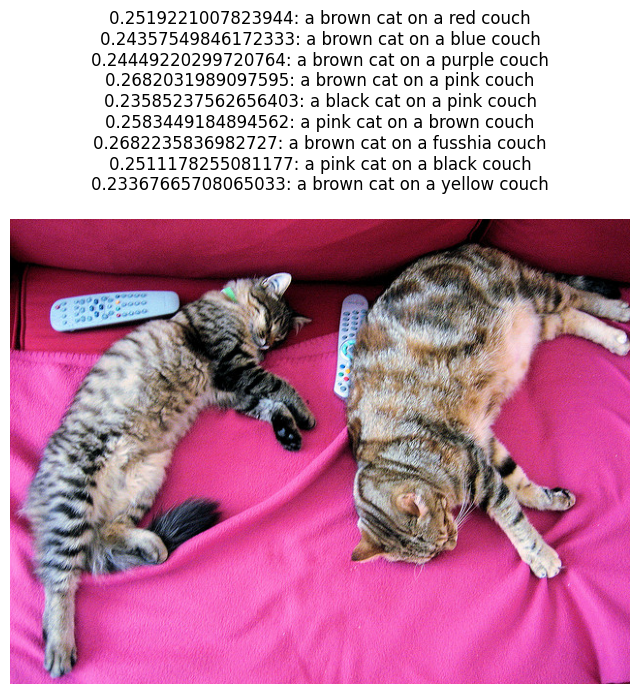
\includegraphics[width=\textwidth]{Graphics/clip_color.png}
 \caption{Colores}
 \label{fig:color}
\end{minipage}%
\begin{minipage}{0.45\textwidth}
 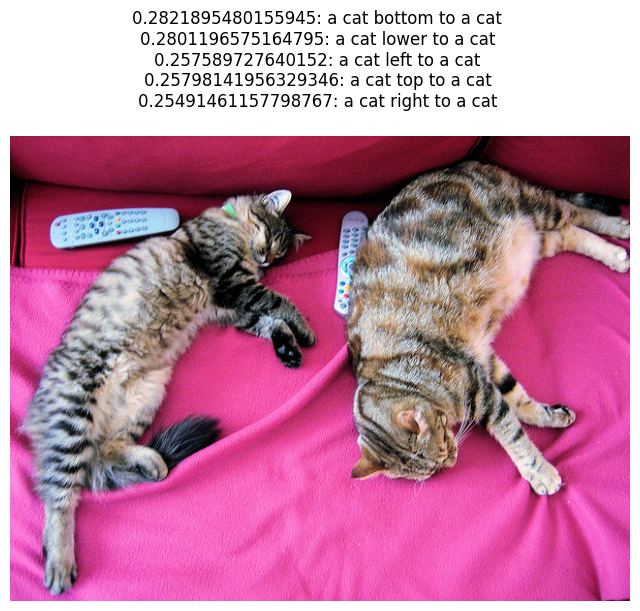
\includegraphics[width=\textwidth]{Graphics/clip_pos.png}
 \caption{Posiciones}
 \label{fig:region}
\end{minipage}
\end{figure}

En las figuras \ref{fig:color} y \ref{fig:region}, se puede observar que el control de colores de CLIP[\cite{clip}] es efectivo, ya que aumenta la similitud a medida que los colores resultan más similares a los de la imagen. Sin embargo, al contrario de las relaciones posicionales, no logra alcanzar la similitud esperada.

El uso de colores a nivel de cuadro de segmentación podría resultar en la selección de colores con una mayor área en la imagen, lo cual no es completamente preciso. Un enfoque más adecuado para esta propuesta de colores sería utilizar las máscaras de segmentación de la imagen con un fondo transparente. Esto podría resultar en una pérdida de precisión en la generación del \textit{embedding}, pero podría conducir a resultados más interesantes que los que CLIP[\cite{clip}] puede manejar actualmente.


\section{Conclusiones de la propuesta}
En esta sección se presenta el resultado de la propuesta final, estableciendo así los parámetros predeterminados para cada función específica, así como los modelos que se decidieron utilizar y la variante que se utiliza por defecto. Cada parámetro es ajustable, probar distintos valores de estos es una opción de experimentación más. Los parámetros predeterminados fueron seleccionados de manera conveniente para los modelos utilizados, de esta manera se asegura un correcto funcionamiento con las similitudes que se obtienen para dichos modelos. En caso de cambiar modelos en el futuro, se recomienda ajustar dichos parámetros para lograr un correcto funcionamiento del sistema. En la Figura \ref{fig:propuestafinal} se muestran las selecciones finales en cuanto a modelos y propuestas, esta elección está sujeta a la disponibilidad de modelos actuales. En trabajos futuros, con el uso de nuevos modelos, el cambio de propuesta puede ser una opción.

\begin{figure}[H]
    \centering
     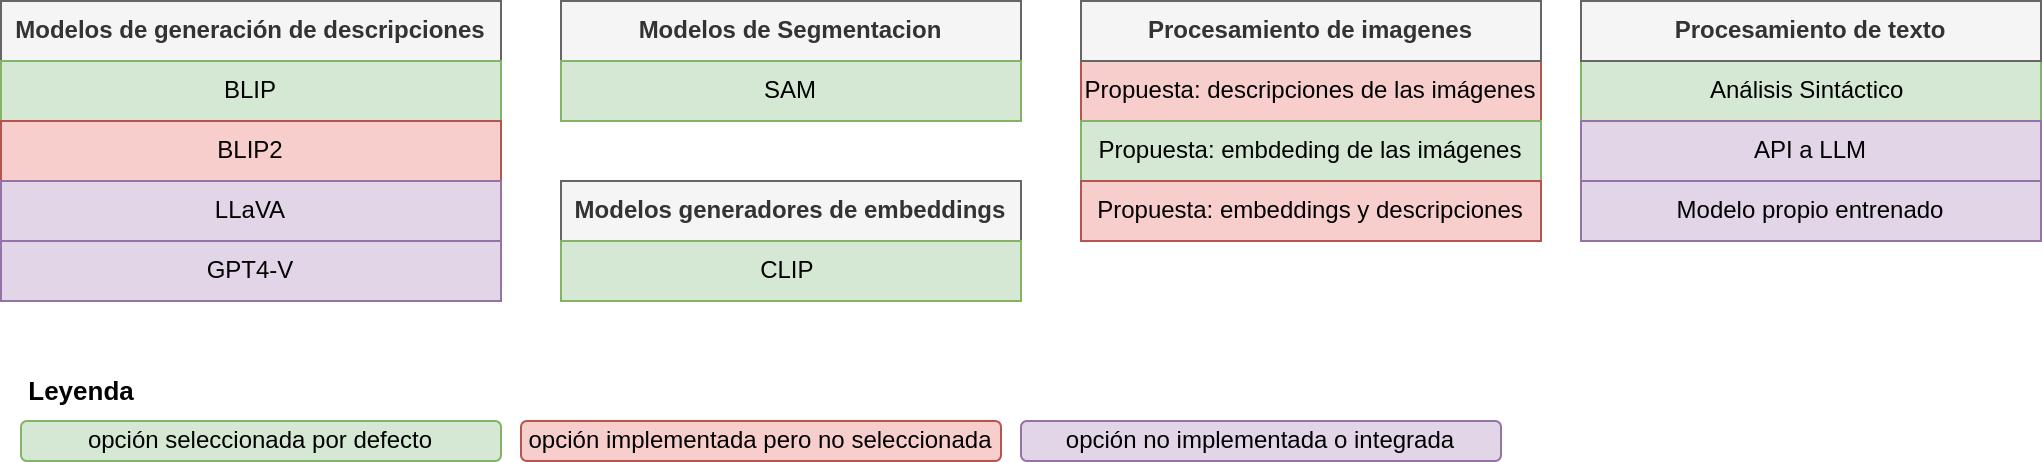
\includegraphics[width=\textwidth]{Graphics/PropuestaFinal.drawio.png}
     \caption{Modelos y propuesta final asignadas por defecto }
\label{fig:propuestafinal}
\end{figure}

\subsection{Entornos(Environments)}
En lo próximo, se dividirá la sección en subsesiones, cada una de las cuales presentará los valores de los parámetros para cada entorno ajustable.

\subsubsection*{SAM Environment}
\begin{itemize}
\item \verb|points-per-side = 32|: define el número de puntos que se utilizan para generar las máscaras. Reducir este número puede acelerar el proceso de segmentación, pero también podría resultar en máscaras menos precisas.
\item \verb|pred-iou-thresh = 0.86|: define el umbral para la intersección sobre la unión (IOU)\supindex{}{Intersection Over Union.} en las predicciones. Aumentar este valor puede resultar en menos regiones propuestas, acelerando el proceso de segmentación.
\item \verb|stability-score-thres = 0.92|: Aumentar este valor puede resultar en menos regiones propuestas.
\item \verb|crop-n-layers = 1|: define el número de capas en el recorte de la imagen. Reducir este número puede acelerar el proceso de segmentación, pero podría afectar negativamente la precisión del modelo.
\item \verb|crop-n-points-downscale-factor = 2|: Aumentar este valor puede resultar en menos puntos en el recorte de la imagen, acelerando el proceso de segmentación.
\item \verb|min-mask-region-area = 20*20|: Aumentar puede resultar en menos regiones propuestas, acelerando el proceso de segmentación, pero pueden perderse segmentaciones importantes.
\end{itemize}

\subsubsection*{\textit{Image Environment}}
\begin{itemize}
\item \verb|USE-CAPION-MODEL = False|: Indica si se usar\'a un modelo de descripciones de im\'agenes para extraer caracter\'isticas.
\item \verb|CAPTION-MODEL = BLIP|: Este es el modelo que se usar\'a para describir la imagen.
\item \verb|CAPTION-IMPORTANCE = 1|: Importancia de la descripci\'on, define que tan importante ser\'a la descripci\'on de una imagen para la similitud. Valor = 1 indica que tiene igual importancia que el embedding de la imagen.
\item \verb|KEY-IMAGES = 'box'|: Esto es el tipo de imagen que usara como principal. (box or mask). \textbf{Box} son todos los p\'ixeles comprendidos en el cuadro de segmentaci\'on donde se ubica un Image. \textbf{Mask} se refiere solo a los p\'ixeles que contienen a la segmentaci\'on dada, el resto ser\'a p\'ixeles en blanco.
\end{itemize}


\subsubsection*{Neighbords Environment}
\begin{itemize}
\item \verb|POS-UMBRAL = 1.2|: Importancia dada a la distancia entre las posiciones de las imagenes. Mientras menor valor mayor importancia, se le da a las posiciones.
\item \verb|PRIMARY-POW  = 0.7|: Elevaci\'on a la potencia del eje principal a la hora de calcular distancias por pesos.
\item \verb|SECUNDARY-POW = 1|: Elevaci\'on a la potencia del eje no principal a la hora de calcular distancias por pesos.
\item \verb|MAX-DISTANCE = 0.85|: Distancia m\'axima que puede existir entre dos im\'agenes para ser consideradas vecinas
\end{itemize}

\subsubsection*{Similarity Environment}

\begin{itemize}
\item \verb|EUCLIDEAN-POW-UMBRAL = 1|: Elevar a la potencia la distancia euclieana.
\item \verb|EUCLIDEAN-DIV-UMBRAL = 10|: Dividir la distancia euclideana entre este valor. C\'alculo de similitud por posiciones. 
\item \verb|MIN-SIMILARTY-FOR-REGIONS = 0.24|: Si la similitud es menor que este valor se considera irrelevante.
\item \verb|MIN-NICE-SIMILARITY = 0.24|: Esta es la similitud a partir de la cual se considera relevante un valor.
\item \verb|MIN-NICE-SIMILARITY-ORIGIN = 0.22|: Esta es la similitud a partir de la cual se considera relevante un valor entre la imagen original y el texto original
\item \verb|MIN-NICE-USE-CAPTION-SIMILARITY = 0.65|: Esta es la similitud a partir de la cual se considera relevante un valor a nivel de texto contra texto.
\item \verb|USE-NEGATIVE-REGIONS = True|: Define si las regiones pueden aportar efecto negativo a la similitud, en el caso de la cercan\'ia entre un objeto y otro.
\item \verb|IMPORTANCE-NEGATIVE-REGIONS = 2|: Define qu\'e tan importante es una regi\'on negativa, mientras m\'as alto, m\'as baja ser\'a la similitud para una regi\'on poco relevante.
\end{itemize}

\subsubsection*{SystemRetrieval Environment}
    \begin{itemize}
    \item \verb|MAX_RANK = 1000|: tamaño m\'aximo de salida el ranking. Cantidad de im\'agenes recuperadas con similitud del coseno
    \item \verb|MAX_END_RANK = 1000|: tamaño m\'aximo de salida final del sistema de recuperaci\'on.
    \end{itemize}